
\section{预测未来供货量}
\subsection{基于神经网络的供货能力预测}

为了优化订购方案,首先需要确定可能的供应量,因此对筛选后的供货商的供应量进行预测,再据此制定相应的订货方案。
供应商接受订单后,会在自身供货能力范围内,调整供货量以满足订单需要。
当订货量过大时,供应商会仅能提供其最大供应量,因此往年供应数据可以反映出供应商的供货能力上限,本文依据供应商历史供应情况来预测其未来供应情况。

订货商的供应量受多种不可控因素影响,若仅根据时间变量构建时间序列预测模型,难以准确拟合供应量曲线,预测效果差。若将其做主要影响因素的回归分析,由于影响因素众多且相互耦合,无法综合分析,与此同时,预测过程中也有预测函数难以构建的问题\cite{李鹏2018基于长短期记忆的实时电价条件下智能电网短期负荷预测}。
%如何预测?

% 调整位置
% 通过分析往年交易数据,本文发现往年供应数据可以反映供应商的供货能力上限。
% 当订货量大于供应能力上限时,供应商无法供应更多的原材料,导致供应量少于订货量。

对于复杂的长时间序列预测的问题,相比于传统时间序列预测手段,深度学习方法有着更好的拟合与预测能力。
深度学习模型是一种拥有多个非线性映射层级的深度神经网络模型,能够对输入信号逐层抽象并提取特征,挖掘出更深层次的潜在规律\cite{lecun2015deep}。
其中,LSTM模型弥补了循环神经网络的梯度消失和梯度爆炸、长期记忆能力不足等问题,使得循环神经网络能够真正有效地利用长距离的时序信息\cite{王鑫2018基于}。

因此,本文使用LSTM分别对选中的44家公司的供货量进行预测。
% 经过测试,本文认为近五年供应商在接受企业的订单后,往往尽其最大努力供货。
% 自然地,这种情况下供应商的供货量主要受其历史供货情况影响,故神经网络不依赖订货量便能够对其进行预测是可以理解的。
本文在过去五年的交易数据中,以前四年训练神经网络,取第五年为测试集。

LSTM是由一系列节点(又称LSTM单元)组成的。如图???所示,LSTM单元内部主要有三个阶段。
在第$t$个节点中:
\\
(1)忘记阶段——对上一个节点的输入进行选择性忘记,即遗忘门
\begin{equation}
    f^{t}=\sigma\left(\omega^{f} \begin{array}{l}
x^t \\
h^{t-1}
\end{array}\right).
\end{equation}
该阶段通过Sigmoid函数,计算得到的$f^{t}$是一个向量,且每个分量均属于$[0,1]$。
一般分量的值会极其接近0或1,为后续选择$c^{t-1}$中用于计算$c^t$的特征做准备。
\\
(2)记忆阶段——选择有效的输入值,即输入门
\begin{equation}
    i^{t}=\sigma\left(\omega^{i} \begin{array}{r}
x^t \\
h^{t-1}
\end{array}\right).
\end{equation}
该阶段工作原理与忘记阶段类似,将用于对输入的$x^t$进行选择。
\\
(3)选择阶段——选择输出并放缩,即输出门
\begin{equation}
    o^{t}=\sigma\left(\omega^{o} \begin{array}{r}
x^t \\
h^{t-1}
\end{array}\right).
\end{equation}
本阶段得到的$o^{t}$会放缩$c^t$,进而决定节点的输出

LSTM的优势是前一节点的状态将随数据一起传入后一节点,但并不向外输出,具体来说也有三个:
\\
(1)单元状态更新值
\begin{equation}
    \check{c}^t=\sigma\left(\omega^{c} \begin{array}{l}
x^t \\
h^{t-1}
\end{array}\right).
\end{equation}
事实上,单元状态更新值与遗忘门、输入门和输出门的作用类似,而且并不传入后一节点。
\\
(2)单元状态
\begin{equation}
c^t=f^tc^{t-1}+i^t\check{c}^t
\end{equation}
\\
(3)隐藏状态
\begin{equation}
   h^t=o^ttanh(c^t)
\end{equation}
最终节点的输出$y^t$也是由$h^t$变化而成的,本文使用的是
\begin{equation}
y^t=\sigma(\omega'h^t)
\end{equation}


本文的LSTM是由PyTorch实现的,可由图???表示……(后续解释用詹桑的md补全。注意讲清具体输入输出时的$x^t$会代入什么?$y^t$是什么,有什么含义?)


\begin{center} {\centering
\vbox{
	\centerline{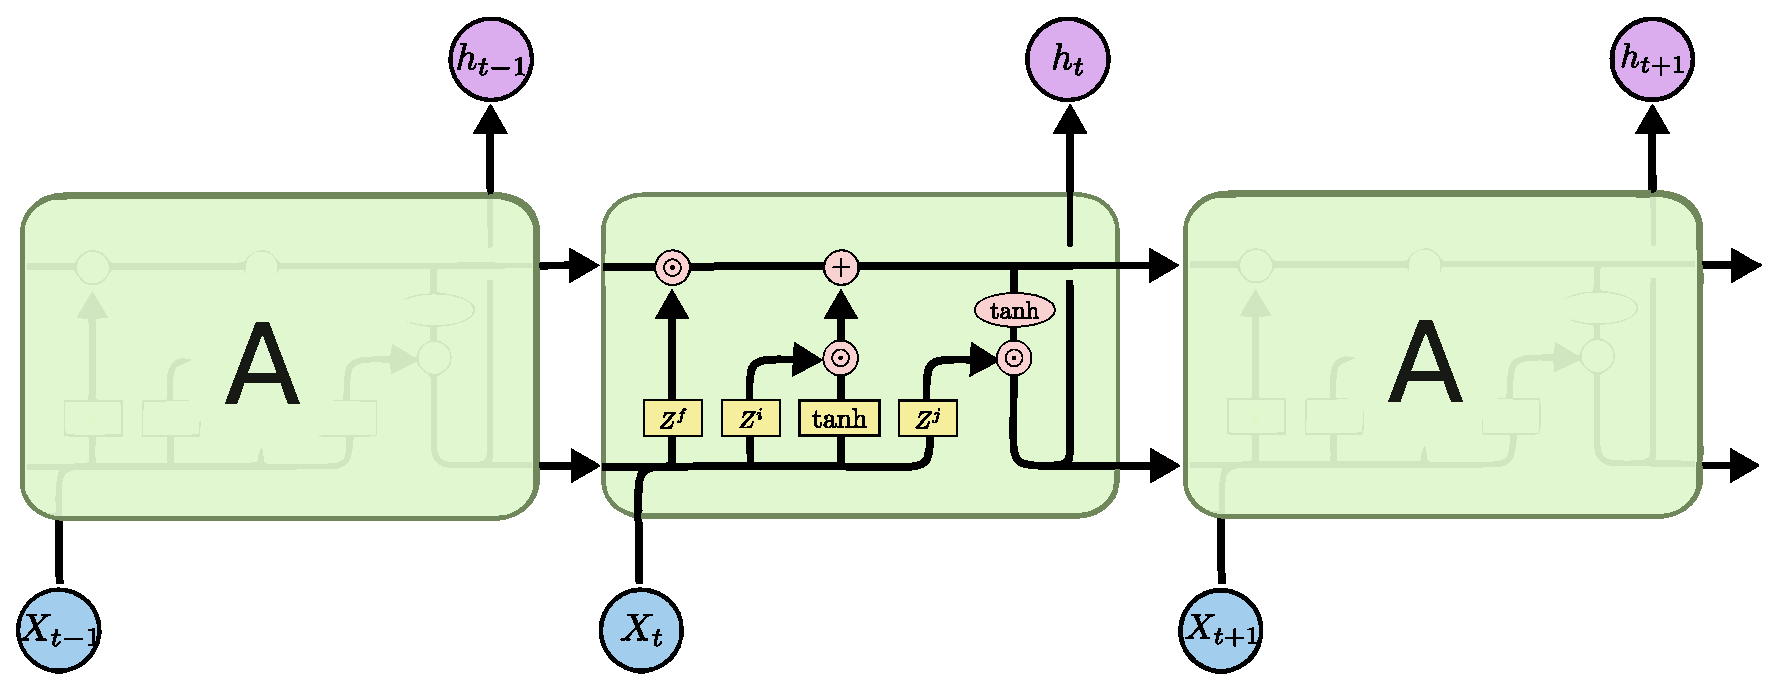
\includegraphics[width=16cm]{Image/lstm.eps}}
	\vskip 1mm{\small
	图2\quad LSTM网络结构图\label{lstm}
	\\
	Fig.\,2\quad LSTM network structure diagram }
	}
	}
\end{center}

%而第$\omega$个节点输出的,即为预测值$\hat{y}_{\omega,n}$,其能反映第$n$家供货商在第$\omega$周的供货能力。

通过分析往年交易数据,供应商总是根据企业订货量来供应原材料。
由于没有考虑提高订购量对供应量的影响,仅根据往年交易数据进行预测,模型对供应商实际供应的预测值会偏小。
通过对预测结果的检验,预测中筛选得到的供应商的总供应量确实小于预期。

\subsection{供应量修正}

% 事实上,某些供应商的供货量由于长期受到订货量的压制而没有体现出应有的供货水平,因此预测量也不能充分说明其供货能力。
% 对于这些供应商,其实际供货能力是高于预测量的,本文引入修正来提升预测量以逼近其真实供货能力。

为了提高预测的准确性,本文为模型添加了反映订货量影响的修正。
数据显示,一定范围内,供应商的供应量会随订货量的增加而增多。
而当订货量超出其的供应能力后,供应商的供货量限于生产条件达到其最大值,即最大供应量。

%未提及仅对部分供应商进行修正!!!

% 若某周的供货量显著低于订货量,则该周的供货量可以较好地反映该周的供货能力,
% 且一般该周的供货量也较多。
进而定义该家供货商的修正比$\alpha_j$:
\begin{equation}
    \alpha_j=\frac{\beta_j-\gamma_j}{\gamma_j}
\end{equation}
\noindent 在第$j$家供应商的历史数据中,当供货量超过订货量时供货量的平均值记为$B_n$,而$c_n$为当供货量小于订货量时供货量的平均值。

修正后第$j$家供货商在第$i$周的实际供货能力$\hat{\psi}_{ij} = \alpha_j y^i_j$。


\subsection{预测模型检验}

本文基于企业前四年的供应数据,建立如上原材料供应量预测模型,并将模型预测结果与真实数据比较以检验模型预测准确性,如下图所示:%图是怎么做的,可以再描述清楚些

\begin{center} {\centering
\vbox{
	\centerline{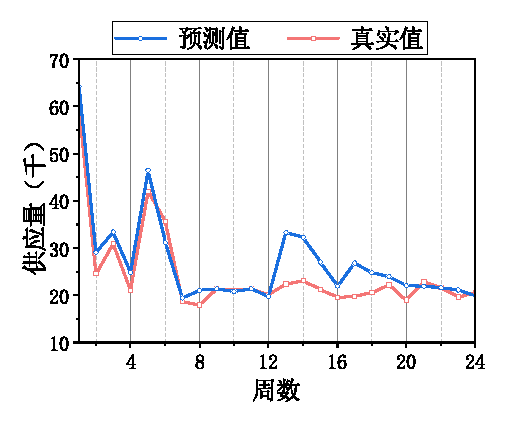
\includegraphics[width=8cm]{Image/comparison.eps}}
	\vskip 1mm{\small
	图2\quad 拟合验证图\label{lstm}
	\\
	Fig.\,2\quad Comparison }
	}
	}
\end{center}

拟合效果较好,故采取该预测模型以预测供应商供货量。%怎么个好法?有定量的表述方法吗?可以再多分析一些

% 最后,本文在共五年的数据中,选择了前四年为训练集,第五年为测试集。在检验预测准确性的同时,也得到了供货量的绝对偏差。经过统计,得到了每家供应商的绝对偏差的期望值$\delta_n$,并用于指导下文的优化模型。